\section{Three flavors of raking}

There are three issues with raking that we are interested in:

\begin{enumerate}
    \item Current raking is done using only the estimated means of the metric that we are interested in. However, we are also given draws (from which we can compute a standard deviation). It would be better to incorporate this information into the raking algorithm, to make sure that values with low uncertainty are only slightly modified whereas values with high uncertainty can vary over a wider range.
    \item It looks like we are doing iterations on the rows and the columns until convergence (IPF?). It would be better to have a common framework for 1D, 2D and 3D raking with different partial sums known.
    \item The raking could be done on absolute numbers (like number of deaths) or on prevalence (like percentage of people with high BMI). In the case of prevalence, we need to ensure that the raked values stay between 0 and 1.
\end{enumerate}

\section{First attempt at naive raking}

\subsection{1D raking problem with and without uncertainties on the means}

Let suppose that we have $n$ independent variables following a distribution $\mathcal{L} \left(\mu_i , \sigma_i \right)$. $\mathcal{L}$ is the same for all variables (e.g. the lognormal distribution) but $\mu_i$ and $\sigma_i$ are different for each variable.

We also know that:

\begin{equation*}
\sum_{i = 1}^n \mu_i = \mu
\end{equation*}

where $\mu$ is known. The $\mu_i$ are unknown but the $\sigma_i$ are known. For each variable $X_i$, we observe only one observation $x_i$. We want to find the coefficients $\alpha_i$ such that $\mu_i = \alpha_i x_i$ for all $i = 1 , \cdots , n$.

\subsubsection{Solution without the $\sigma_i$}

In the first case, we do not use the $\sigma_i$ and we assume that all the $\alpha_i$ are equal. We thus look for $\alpha$ such that:

\begin{equation*}
\sum_{i = 1}^n \mu_i = \sum_{i = 1}^n \alpha x_i = \mu
\end{equation*}

which gives us:

\begin{equation}
\alpha = \frac{\mu}{\sum_{i = 1}^n x_i}
\end{equation}

We can also write this problem as an optimization problem. We want to minimize the Kullback-Leibler divergence:

\begin{equation*}
\sum_{i = 1}^n \alpha_i x_i \log \left( \alpha_i \right)
\end{equation*}

under the constraint:

\begin{equation*}
\sum_{i = 1}^n \alpha_i x_i = \mu
\end{equation*}

We write the Lagrangian:

\begin{equation*}
\mathcal{L} \left( \alpha_i, \lambda \right) = \sum_{i = 1}^n \alpha_i x_i \log \left( \alpha_i \right) + \lambda \left( \sum_{i = 1}^n \alpha_i x_i - \mu \right)
\end{equation*}

Taking the derivatives with respect to the $\alpha_i$, we get:

\begin{equation*}
\frac{\partial \mathcal{L} \left(\alpha_j , \lambda \right)}{\partial \alpha_i} = x_i \left( \log \alpha_i + 1 \right) + \lambda x_i = 0
\end{equation*}

which gives us:

\begin{equation*}
\alpha_i = \exp \left( - 1 - \lambda \right)
\end{equation*}

Using the constraint, we have:

\begin{equation*}
\sum_{i = 1}^n x_i \exp \left( - 1 - \lambda \right) = \mu
\end{equation*}

which gives us:

\begin{equation*}
- 1 - \lambda = \log \left( \frac{\mu}{\sum_{i = 1}^n x_i} \right)
\end{equation*}

Finally we get:

\begin{equation*}
\alpha_i = \frac{\mu}{\sum_{j = 1}^n x_j}
\end{equation*}

that is we get back to the initial solution.

\subsubsection{Solution with the $\sigma_i$}

In the second case, we use the $\sigma_i$ and we assume that:

\begin{equation*}
\frac{\alpha_i - 1}{\sigma_i} = \frac{\alpha_j - 1}{\sigma_j} \text{ for all } 1 \leq i < j \leq n
\end{equation*}

It gives us:

\begin{equation*}
\frac{\alpha_i - 1}{\sigma_i} = C \text{ for all } i = 1 , \cdots , n
\end{equation*}

Using the constraint on the sum, we get:

\begin{equation*}
\sum_{i = 1}^n \alpha_i x_i = \sum_{i = 1}^n \left( C \sigma_i + 1 \right) x_i = C \left( \sum_{i = 1}^n \sigma_i x_i \right) + \sum_{i = 1}^n x_i = \mu
\end{equation*}

that is:

\begin{equation*}
C = \frac{\mu - \sum_{i = 1}^n x_i}{\sum_{i = 1}^n \sigma_i x_i}
\end{equation*}

Finally, we get:

\begin{equation*}
\alpha_i = 1 + \sigma_i \frac{\mu - \sum_{j = 1}^n x_j}{\sum_{j = 1}^n \sigma_j x_j}
\end{equation*}

\subsubsection{Solution without the assumption on the $\frac{\alpha_i - 1}{\sigma_i}$}

In a more complex version of the problem, instead of assuming that:

\begin{equation*}
\frac{\alpha_i - 1}{\sigma_i} = \frac{\alpha_j - 1}{\sigma_j} \text{ for all } 1 \leq i < j \leq n
\end{equation*}

we try to minimize:

\begin{equation*}
\sum_{i = 1}^n \left( \frac{\alpha_i - 1}{\sigma_i} \right) ^2
\end{equation*}

under the constraint:

\begin{equation*}
\sum_{i = 1}^n \alpha_i x_i = \mu
\end{equation*}

We write the Lagrangian:

\begin{equation*}
\mathcal{L} \left( \alpha_i , \lambda \right) = \sum_{i = 1}^n \left( \frac{\alpha_i - 1}{\sigma_i} \right) ^2 - \lambda \left( \sum_{i = 1}^n \alpha_i x_i - \mu \right)
\end{equation*}

and get:

\begin{equation*}
\frac{\partial \mathcal{L} \left( \alpha_i , \lambda \right)}{\partial \alpha_i} = 2 \frac{\alpha_i - 1}{\sigma_i} - \lambda x_i = 0
\end{equation*}

that is:

\begin{equation*}
\alpha_i = 1 + \lambda \frac{x_i \sigma_i}{2}
\end{equation*}

Using the constraint, we get:

\begin{equation*}
\mu = \sum_{i = 1}^n \alpha_i x_i = \sum_{i = 1}^n \left( 1 + \lambda \frac{x_i \sigma_i}{2} \right) x_i
\end{equation*}

which gives us:

\begin{equation*}
\lambda = \frac{\mu - \sum_{i = 1}^n x_i}{\sum_{i = 1}^n \frac{x_i^2 \sigma_i}{2}}
\end{equation*}

and the final solution:

\begin{equation*}
\alpha_i = 1 + x_i \sigma_i \frac{\mu - \sum_{j = 1}^n x_j}{\sum_{j = 1}^n x_j^2 \sigma_j}
\end{equation*}

\textit{Note:}
As long as $\mu > \sum_{i = 1}^n x_i$, we won't have negative values for the raking. In the case where $\mu < \sum_{i = 1}^n x_i$, the condition on the $\mu$, $x_i$ and $\sigma_i$ becomes more complex. We may want to add the inequality constraints $\alpha_i > 0$ to the optimization problem.

\subsubsection{Comparison between the 3 methods}

To be able to compare the three methods, we choose the values $\mu$, $\mu_i$ and $\sigma_i$. Then we do $N$ simulations.

For each simulation $j$, we draw a single value $x_i^j$ for each of the $n$ distributions $\mathcal{L} \left( \mu_i , \sigma_i \right)$. Then we compute the corresponding values:

\begin{equation*}
\tilde{\mu}_i^j = \alpha_i^j x_i^j
\end{equation*}

for each of the three raking methods.

For each variable $X_i$, we can compute the Mean Average Percentage Error (MAPE):

\begin{equation*}
e_i = \frac{1}{N} \sum_{j = 1}^N \frac{\left\vert \mu_i - \tilde{\mu}_i^j \right\vert}{\mu_i}
\end{equation*}

and the mean error over all variables:

\begin{equation*}
e = \frac{1}{n} \sum_{i = 1}^n \left( \frac{1}{N} \sum_{j = 1}^N \frac{\left\vert \mu_i - \tilde{\mu}_i^j \right\vert}{\mu_i} \right)
\end{equation*}

We take $\mu_i = 0.1$ for $i = 1 , \cdots , 9$, $\mu = 1$, $\sigma_9 = 0.1$ and $\sigma_{i - 1} = \sigma_{i} / 2$ for $i = 2 , \cdots , 9$. We choose a lognormal distribution and we do 500 simulations. The corresponding MAPE for each variable and each raking method is shown on Figure 1. Using or not the assumption on the $\frac{\alpha_i - 1}{\sigma_i}$ does not seem to have much effect. For the variables with small variance, using the standard deviation for the raking greatly improves the result. This is not the case for the variables with high standard deviation. This is illustrated in Figure 2, which shows the MAPE as a function of the standard deviation for each raking method.

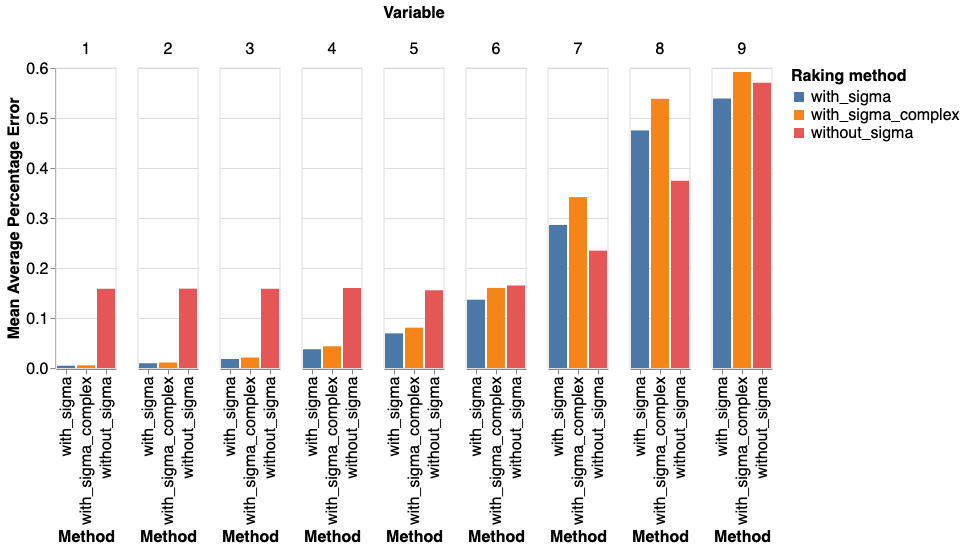
\includegraphics[width=15cm]{projects/raking/figures/MAPE_variable.png}
\captionof{figure}{Mean Average Percentage Error (MAPE) for each variable for the three raking methods.}

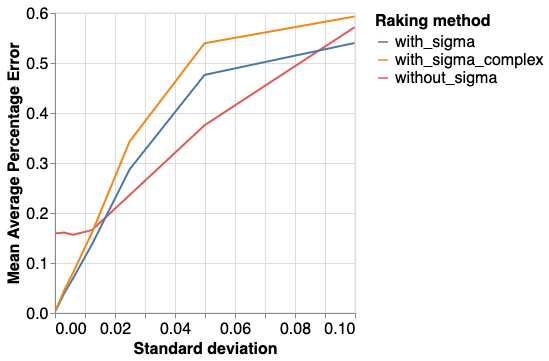
\includegraphics[width=15cm]{projects/raking/figures/MAPE_standard_deviation.png}
\captionof{figure}{Mean Average Percentage Error (MAPE) as a function of the standard deviation of the variable for the three raking methods.}

The code for the simulation is located here: \href{https://github.com/ADucellierIHME/raking_1Dtoy}{1D raking code}.

\subsection{2D raking problem with and without uncertainties on the means}

Let suppose that we have $n * m$ independent variables following a distribution $\mathcal{L} \left(\mu_{i,j} , \sigma_{i,j} \right)$. $\mathcal{L}$ is the same for all variables (e.g. the lognormal distribution) but $\mu_{i,j}$ and $\sigma_{i,j}$ are different for each variable.

We also know that:

\begin{equation*}
\sum_{i = 1}^n \mu_{i,j} = \mu_{.j} \text{ and } \sum_{j = 1}^m \mu_{i,j} = \mu_{i.}
\end{equation*}

where the $\mu_{i.} , i = 1 ,\cdots , n$ and the $\mu_{.j} , j = 1 , \cdots , m$ are known. The $\mu_{i,j}$ are unknown but the $\sigma_{i,j}$ are known. For each variable $X_{i,j}$, we observe only one observation $x_{i,j}$. We want to find the coefficients $\alpha_{i,j}$ such that $\mu_{i,j} = \alpha_{i,j} x_{i,j}$ for all $i = 1 , \cdots , n$ and $j = 1 , \cdots , m$.

\subsubsection{Solution without the $\sigma_{i,j}$}

In the first case, we do not use the $\sigma_{i,j}$. As we have done for the 1D case, we want to minimize the Kullback-Leibler divergence:

\begin{equation*}
\sum_{i = 1}^n \sum_{j = 1}^m \alpha_{i,j} x_{i,j} \log \left( \alpha_{i,j} \right)
\end{equation*}

under the constraints:

\begin{align*}
\sum_{i = 1}^n \alpha_{i,j} x_{i,j} &= \mu_{.j} \text{ for } j = 1 , \cdots , m \\
\sum_{j = 1}^m \alpha_{i,j} x_{i,j} &= \mu_{i.} \text{ for } i = 1 , \cdots , n
\end{align*}

We can use Iterative Proportional Fitting (IPF) to solve the problem.

\vspace{1em}

\textbf{Iterative Proportional Fitting}

\vspace{1em}

We observe $m * n$ values $x_{i,j}$ for $i = 1 , \cdots , n$ and $j = 1 , \cdots , m$ and the total sum $\mu$. We want to find the weights $\alpha_{i,j}$ such that:

\begin{equation*}
\mu = \sum_{i = 1}^n \sum_{j = 1}^m \mu_{i,j} = \sum_{i = 1}^n \sum_{j = 1}^m \alpha_{i,j} x_{i,j}
\end{equation*}

We also know the partial sums:

\begin{align*}
\sum_{i = 1}^n \alpha_{i,j} x_{i,j} &= \mu_{.j} \text{ for } j = 1 , \cdots , m \\
\sum_{j = 1}^m \alpha_{i,j} x_{i,j} &= \mu_{i.} = \text{ for } i = 1 , \cdots , n
\end{align*}

where the $\mu_{.j}$ and the $\mu_{i.}$ are known values such that:

\begin{equation*}
\sum_{j = 1}^m \mu_{.j} = \mu \text{ and } \sum_{i = 1}^n \mu_{i.} = \mu
\end{equation*}

This is an optimization problem where we want to minimize the Kullback-Leibler divergence:

\begin{equation*}
\sum_{i = 1}^n \sum_{j = 1}^m \alpha_{i,j} x_{i,j} \log \left( \alpha_{i,j} \right)
\end{equation*}

under the constraints:

\begin{align*}
\sum_{i = 1}^n \alpha_{i,j} x_{i,j} &= \mu_{.j} \text{ for } j = 1 , \cdots , m \\
\sum_{j = 1}^m \alpha_{i,j} x_{i,j} &= \mu_{i.} \text{ for } i = 1 , \cdots , n
\end{align*}

We can compute the Lagrangian:

\begin{equation*}
\mathcal{L} \left( \alpha_{i,j} , \lambda_j , \nu_i \right) = \sum_{i = 1}^n \sum_{j = 1}^m \alpha_{i,j} x_{i,j} \log \left( \alpha_{i,j} \right) + \sum_{j = 1}^m \lambda_j \left( \sum_{i = 1}^n \alpha_{i,j} x_{i,j} - \mu_{.j} \right) + \sum_{i = 1}^n \nu_i \left( \sum_{j = 1}^m \alpha_{i,j} x_{i,j} - \mu_{i.} \right)
\end{equation*}

taking the derivatives with respect to the $\alpha_{i,j}$, we get:

\begin{equation*}
\frac{\partial \mathcal{L} \left( \alpha_{i,j}, \lambda_j , \nu_i \right)}{\partial \alpha_{i,j}} = x_{i,j} \left( \log \left( \alpha_{i,j} \right) + 1 \right) + \lambda_j x_{i,j} + \nu_i x_{i,j} = 0
\end{equation*}

which gives us:

\begin{equation*}
\alpha_{i,j} = e^{-\frac{1}{2} - \lambda_j} e^{-\frac{1}{2} - \nu_i}
\end{equation*}

It means that $\alpha_{i,j}$ is the product of a scalar that depends only on the row $i$ and a scalar that depends only on the column $j$. In order to find the values of the $\nu_i$ and $\lambda_j$, we use an iterative procedure. At the iteration $k = 0$, we start with:

\begin{equation*}
\alpha_{i,j}^{\left(0\right)} = 1
\end{equation*}

Then we alternate between odd and even iterations. We start by multiplying each column by a different scalar (to get the $\lambda_j$):

\begin{equation}
\alpha_{i,j}^{\left(2 k - 1\right)} = \alpha_{i,j}^{\left(2 k - 2\right)} \frac{\mu_{.j}}{\sum_{i = 1}^n \alpha_{i,j}^{\left(2 k - 2\right)} x_{i,j}}
\end{equation}

Then we multiply each row by a different scalar (to get the $\nu_i$):

\begin{equation}
\alpha_{i,j}^{\left(2 k\right)} = \alpha_{i,j}^{\left(2 k - 1\right)} \frac{\mu_{i.} }{\sum_{j = 1}^m \alpha_{i,j}^{\left(2 k - 1\right)} x_{i,j}}
\end{equation}

We stop the iterations when the difference between the $\alpha_{i,j}^{\left(k\right)}$ and the $\alpha_{i,j}^{\left(k - 1\right)}$ becomes very small.

In the log domain, we can reformulate the algorithm as:

\begin{equation*}
\beta_{i,j}^{\left(0\right)} = \log \alpha_{i,j}^{\left(0\right)} = 0
\end{equation*}

with:

\begin{equation*}
\beta_{i,j}^{\left(2 k - 1\right)} = \beta_{i,j}^{\left(2 k - 2\right)} + \log \mu_{.j} - \log \left( \sum_{i = 1}^n x_{i,j} \exp \left( \beta_{i,j}^{\left(2 k - 2\right)} \right) \right)
\end{equation*}

and:

\begin{equation*}
\beta_{i,j}^{\left(2 k\right)} = \beta_{i,j}^{\left(2 k - 1\right)} + \log \mu_{i.} - \log \left( \sum_{j = m}^n x_{i,j} \exp \left( \beta_{i,j}^{\left(2 k - 1\right)} \right) \right)
\end{equation*}

\vspace{1em}

\textbf{Application}

\vspace{1em}

Iterative Proportional Fitting is implemented here: \href{https://github.com/ADucellierIHME/raking_IPF}{IPF and example}. As an example, we sample $n * m$ values from an uniform distribution over the interval $\left[ \frac{0.01}{n m}, \frac{1.99}{n m} \right]$ for the $x_{i,j}$. We sample $n$ values from an uniform distribution over the interval $\left[ \frac{0.75}{n} , \frac{1.25}{n} \right]$ for the $\mu_{i.}$ and we normalize so that the sum adds up to 1. We sample $m$ values from an uniform distribution over the interval $\left[ \frac{0.75}{m}, \frac{1.25}{m} \right]$ for the $\mu_{.j}$ and we normalize so that the sum adds up to 1. We iterate until the average:

\begin{equation*}
\frac{1}{n m} \sum_{i = 1}^n \sum_{j = 1}^m \left\vert \frac{\alpha_{i,j}^{\left( k - 1 \right)} - \alpha_{i,j}^{\left( k \right)}}{(\alpha_{i,j}^{\left( k - 1 \right)}} \right\vert
\end{equation*}

is smaller than $1.0 * 10^{-10}$. At each iteration, we compute:

\begin{equation*}
\frac{1}{2} \left( \frac{1}{m} \sum_{j = 1}^m \left\vert \mu_{.j} - \sum_{i = 1}^n \alpha_{i,j} x_{i,j} \right\vert + \frac{1}{n} \sum_{i = 1}^n \left\vert \mu_{i.} - \sum_{j = 1}^m \alpha_{i,j} x_{i,j} \right\vert \right)
\end{equation*}

For $n = 50$ and $m = 40$, we show the convergence with the initial formulation in Figure 3 and the convergence with the log formulation (implemented with Torch tensors instead of Numpy arrays) in Figure 4. The log formulation should give exactly the same result, but may be more numerically stable if we have low values in the exponentials.

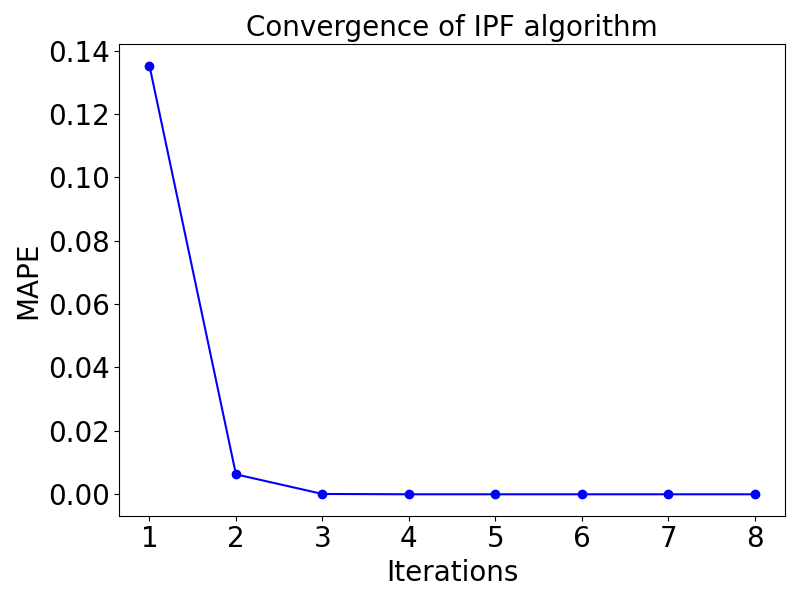
\includegraphics[width=15cm]{projects/raking/figures/IPF_convergence.png}
\captionof{figure}{Mean Absolute Error (MAE) between actual partial sums and raked partial sums at each iteration for the initial formulation.}

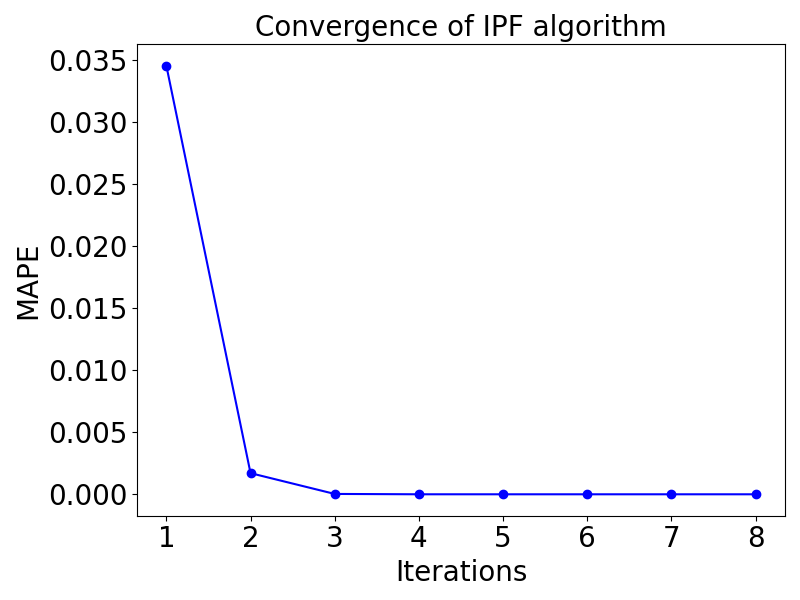
\includegraphics[width=15cm]{projects/raking/figures/IPF_torch_convergence.png}
\captionof{figure}{Mean Absolute Error (MAE) between actual partial sums and raked partial sums at each iteration for the log formulation.}

We now test several values of $n$ and $m$ to compare the computation time. The number of iterations and the computation time as a function of the number of values in  the matrix to be raked is shown in Figure 5.

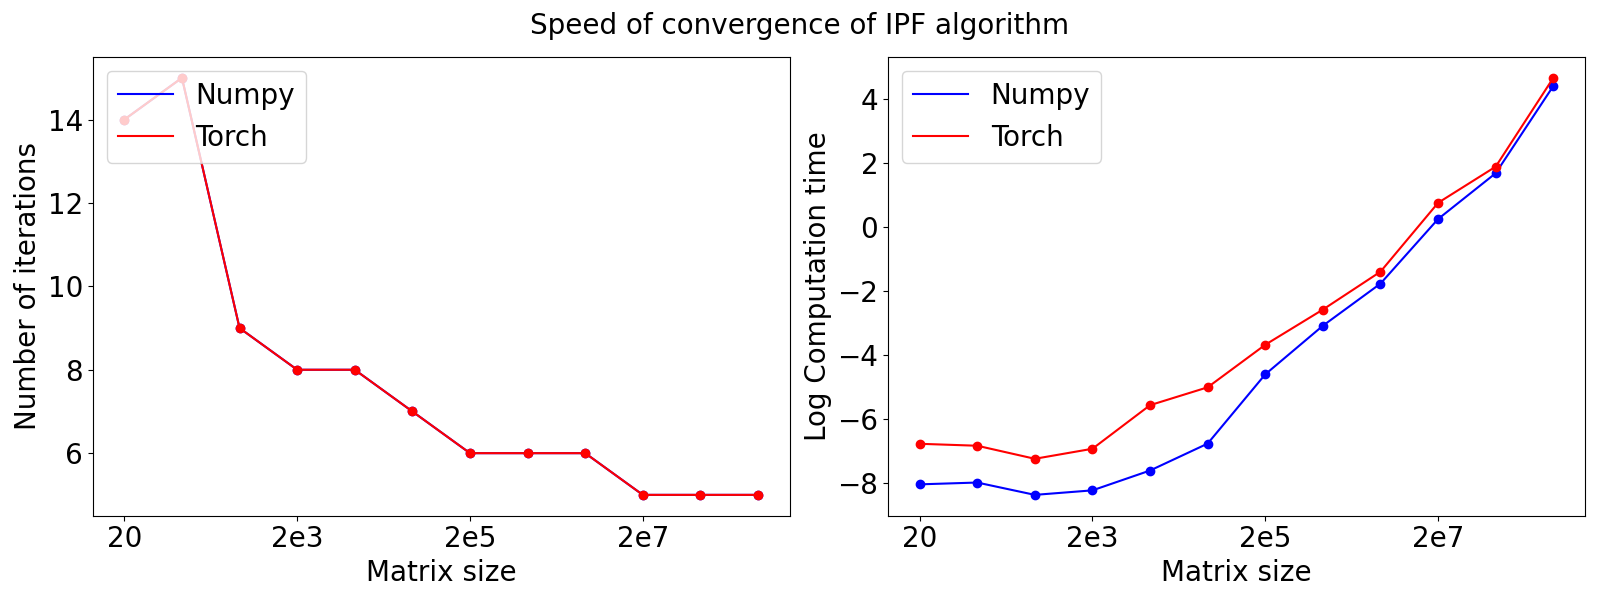
\includegraphics[width=15cm]{projects/raking/figures/IPF_convergence_speed.png}
\captionof{figure}{Number of iterations (left) and computation time (right) as a function of the size of the matrix for the Numpy and the Torch implementations.}

The computation times are similar when the raked matrix becomes big, so we may use the log formulation to avoid numerical problems with small values.

\subsubsection{Solution with the $\sigma_{i,j}$}

We are going to introduce a penalty in the optimization problem. We now want to minimize:

\begin{equation*}
\sum_{i = 1}^n \sum_{j = 1}^m \left( \alpha_{i,j} + C \sigma_{i,j} \right) x_{i,j} \log \left( \alpha_{i,j} + C \sigma_{i,j} \right)
\end{equation*}

under the constraints:

\begin{align*}
\sum_{i = 1}^n \alpha_{i,j} x_{i,j} &= \mu_{.j} \text{ for } j = 1 , \cdots , m \\
\sum_{j = 1}^m \alpha_{i,j} x_{i,j} &= \mu_{i.} \text{ for } i = 1 , \cdots , n
\end{align*}

Using the same formulation as in the 1D case won't work well, it will be easier to use something like:

\begin{equation*}
\sum_{i = 1}^n \sum_{j = 1}^m w_{i,j} \left( \sigma_{i,j} \right) \alpha_{i,j} x_{i,j} \log \left( \alpha_{i,j} \right)
\end{equation*}

\section{Definition of the raking problem(s)}

\subsection{1D case}

\subsubsection{The linear case}

If we define $N$ the number of cases in the entire group and $X_i$ the number of cases in the sub-group $i$ with $i = 1 , \cdots , n$. We assume that $N$ follows some distribution:

\begin{equation*}
N \sim \left( \mu , \sigma \right) \text{ with draws } d_j , j = 1 , \cdots , m
\end{equation*}

Similarly, the $X_i$ follow some distributions:

\begin{equation*}
X_i \sim \left( \mu_i , \sigma_i \right) \text{ with draws } d_{i,j} , j = 1 , \cdots , m
\end{equation*}

We suppose that $\mu$ is known and that for each variable $X_i$, we have one observation $N_i$. We want to find estimates $\tilde{\mu}_i = r_i N_i$ of the $\mu_i$ such that:

\begin{equation*}
\mu = \sum_{i = 1}^n \tilde{\mu}_i = \sum_{i = 1}^n r_i N_i
\end{equation*}

One simple solution is to have:

\begin{equation*}
r_i = \frac{\mu}{\sum_{k = 1}^n N_k} \text{ for } i = 1 , \cdots , n
\end{equation*}

For the draws, the problem is similar and we get the weights:

\begin{equation*}
r_{i,j} = \frac{d_j}{\sum_{k = 1}^n d_{k,j}} \text{ for } i = 1 , \cdots , n \text{ and } j = 1 , \cdots , m
\end{equation*}

\subsubsection{The logit case}

\subsection{2D case}

We observe $m * n$ values $\mu_{i,j}$ for $i = 1 , \cdots , n$ and $j = 1 , \cdots , m$ and the total sum $N$. We want to find the weights $r_{i,j}$ such that:

\begin{equation*}
N = \sum_{i = 1}^n \sum_{j = 1}^m N_{i,j} = \sum_{i = 1}^n \sum_{j = 1}^m r_{i,j} \mu_{i,j}
\end{equation*}

We also know the partial sums:

\begin{align*}
\sum_{i = 1}^n r_{i,j} \mu_{i,j} &= N_{.j} = f_{.j} N \text{ for } j = 1 , \cdots , m \\
\sum_{j = 1}^m r_{i,j} \mu_{i,j} &= N_{i.} = f_{i.} N \text{ for } i = 1 , \cdots , n
\end{align*}

where the $f_{.j}$ and the $f_{i.}$ are known values such that:

\begin{equation*}
\sum_{j = 1}^m f_{.j} = 1 \text{ and } \sum_{i = 1}^n f_{i.} = 1
\end{equation*}

\subsubsection{First possibility}

We want to find the $r_{i,j}$ that minimize:

\begin{equation*}
\left( N - \sum_{i = 1}^n \sum_{j = 1}^m r_{i,j} \mu_{i,j} \right) ^2
\end{equation*}

under the $m + n$ constraints:

\begin{align*}
\sum_{i = 1}^n r_{i,j} \mu_{i,j} &= N_{.j} = f_{.j} N \text{ for } j = 1 , \cdots , m \\
\sum_{j = 1}^m r_{i,j} \mu_{i,j} &= N_{i.} = f_{i.} N \text{ for } i = 1 , \cdots , n
\end{align*}

and the $m * n$ constraints:

\begin{equation*}
r_{i,j} > 0 \text{ for all } i = 1 , \cdots , n \text{ and } j = 1 , \cdots , m
\end{equation*}

\subsubsection{Second possibility}

We want to find the $r_{i,j}$ that minimize:

\begin{equation*}
\sum_{j = 1}^m \left( f_{.j} N - \sum_{i = 1}^n r_{i,j} \mu_{i,j} \right) ^2 + \sum_{i = 1}^n \left( f_{i.} N - \sum_{j = 1}^m r_{i,j} \mu_{i,j} \right) ^2
\end{equation*}

under the constraint:
\begin{equation*}
N = \sum_{i = 1}^n \sum_{j = 1}^m r_{i,j} \mu_{i,j}
\end{equation*}

and the $m * n$ constraints:

\begin{equation*}
r_{i,j} > 0 \text{ for all } i = 1 , \cdots , n \text{ and } j = 1 , \cdots , m
\end{equation*}

\subsection{3D case}

We are given $N$, the total number of deaths (all causes) in a given state and the $\mu_{i,j,k}$, the number of deaths from cause $i$, in county $j$ for race $k$ where $i = 1 , \cdots , l$, $j = 1 , \cdots , m$ and $k = 1 , \cdots , n$. We want to find the $r_{i,j,k}$ such that:

\begin{equation*}
N = \sum_{i = 1}^l \sum_{j = 1}^m \sum_{k = 1}^n r_{i,j,k} \mu_{i,j,k}
\end{equation*}

At the state level, we know the number of deaths from a specific cause $i$ (from the GBD), thus we have the $l$ constraints:

\begin{equation*}
\sum_{j = 1}^m \sum_{k = 1}^n r_{i,j,k} \mu_{i,j,k} = N_{i..} = f_{i..} N \text{ for all } i = 1 , \cdots l
\end{equation*}

where the $f_{i..}$ are known values such that:

\begin{equation*}
\sum_{i = 1}^l f_{i..} = 1
\end{equation*}

We also know the total number of deaths (all causes) for each county $j$ and each race $k$, thus we have the $m * n$ constraints:

\begin{equation*}
\sum_{i = 1}^l r_{i,j,k} \mu_{i,j,k} = N_{.jk} = f_{.jk} N \text{ for all } j = 1 , \cdots , m \text{ and } k = 1 , \cdots , n
\end{equation*}

where the $f_{.jk}$ are known values such that:

\begin{equation*}
\sum_{j = 1}^m \sum_{k = 1}^n f_{.jk} = 1
\end{equation*}

Finally, we have the $l * m * n$ constraints:

\begin{equation*}
r_{i,j,k} > 0 \text{ for all } i = 1 , \cdots , l \text{, } j = 1 , \cdots , m \text{ and } k = 1 , \cdots , n
\end{equation*}

\subsection{Analogy with the age-sex splitting problem}

The raking problem is similar to the age-sex splitting problem. In the age-sex splitting problem, we have the total number of deaths $N$ and the total number of people $M$. We want to know the number of deaths $N_{i,j}$ for each age group $i$ and each sex $j$ with $i = 1 , \cdots , m$, $j = 1 , \cdots , n$.

We know the number of people $M_{i,j}$ in each age group and each sex:

\begin{equation*}
M_{i,j} = f_{i,j} M \text{ for } i = 1 , \cdots , m \text{ and } j = 1 , \cdots , n.
\end{equation*}

We know the ratio between the probability $\frac{\sum_{j = 1}^n N_{i_1,j}}{\sum_{j = 1}^n M_{i_1,j}}$ of dying at age $i_1$ and the probability of dying $\frac{\sum_{j = 1}^n N_{i_2,j}}{\sum_{j = 1}^n M_{i_2,j}}$ at age $i_2$:

\begin{equation*}
\frac{\frac{\sum_{j = 1}^n N_{i_1,j}}{\sum_{j = 1}^n M_{i_1,j}}}{\frac{\sum_{j = 1}^n N_{i_2,j}}{\sum_{j = 1}^n M_{i_2,j}}} = \frac{\sum_{j = 1}^n N_{i_1,j}}{\sum_{j = 1}^n N_{i_2,j}} \frac{\sum_{j = 1}^n M_{i_2,j}}{\sum_{j = 1}^n M_{i_1,j}} = \alpha_{i_1,i_2}
\end{equation*}

We know the ratio between the probability $\frac{\sum_{i = 1}^m N_{i,j_1}}{\sum_{i = 1}^m M_{i,j_1}}$ of dying for sex $j_1$ and the probability of dying $\frac{\sum_{i = 1}^m N_{i,j_2}}{\sum_{i = 1}^n M_{i,j_2}}$ for sex $j_2$:

\begin{equation*}
\frac{\frac{\sum_{i = 1}^m N_{i,j_1}}{\sum_{i = 1}^m M_{i,j_1}}}{\frac{\sum_{i = 1}^m N_{i,j_2}}{\sum_{i = 1}^m M_{i,j_2}}} = \frac{\sum_{i = 1}^m N_{i,j_1}}{\sum_{i = 1}^m N_{i,j_2}} \frac{\sum_{i = 1}^m M_{i,j_2}}{\sum_{i = 1}^m M_{i,j_1}} = \beta_{i_1,i_2}
\end{equation*}

We want to find the $N_{i,j}$ such that:

\begin{equation*}
\sum_{i = 1}^m \sum_{j = 1}^n N_{i,j} = N
\end{equation*}

\subsubsection{First possibility}

We want to find the $N_{i,j}$ that minimize:

\begin{equation*}
\left( N - \sum_{i = 1}^n \sum_{j = 1}^m N_{i,j} \right) ^2
\end{equation*}

under the $\frac{m \left( m - 1\right)}{2}$ constraints:

\begin{equation*}
\left( \sum_{j = 1}^n N_{i_1,j} \right) \left( \sum_{j = 1}^n M_{i_2,j} \right) = \alpha_{i_1,i_2} \left( \sum_{j = 1}^n N_{i_2,j} \right) \left( \sum_{j = 1}^n M_{i_1,j} \right)
\end{equation*}

the $\frac{n \left( n - 1 \right)}{2}$ constraints:

\begin{equation*}
\left( \sum_{i = 1}^m N_{i,j_1} \right) \left( \sum_{i = 1}^m M_{i,j_2} \right) = \beta_{i_1,i_2} \left( \sum_{i = 1}^m N_{i,j_2} \right) \left( \sum_{i = 1}^m M_{i,j_1} \right)
\end{equation*}

and the $m * n$ constraints:

\begin{equation*}
N_{i,j} > 0 \text{ for all } i = 1 , \cdots , n \text{ and } j = 1 , \cdots , m
\end{equation*}

\subsubsection{Second possibility}

We want to find the $N_{i,j}$ that minimize:

\begin{align*}
&\sum_{i_1 = 1}^{m - 1} \sum_{i_2 = i_1 + 1}^m \left( \left( \sum_{j = 1}^n N_{i_1,j} \right) \left( \sum_{j = 1}^n M_{i_2,j} \right) - \alpha_{i_1,i_2} \left( \sum_{j = 1}^n N_{i_2,j} \right) \left( \sum_{j = 1}^n M_{i_1,j} \right) \right) ^2 + \\
&\sum_{j_1 = 1}^{n - 1} \sum_{j_2 = j_1 + 1}^n \left( \left( \sum_{i = 1}^m N_{i,j_1} \right) \left( \sum_{i = 1}^m M_{i,j_2} \right) - \beta_{i_1,i_2} \left( \sum_{i = 1}^m N_{i,j_2} \right) \left( \sum_{i = 1}^m M_{i,j_1} \right) \right) ^2
\end{align*}

under the constraint:

\begin{equation*}
N = \sum_{i = 1}^n \sum_{j = 1}^m N_{i,j}
\end{equation*}

and the $m * n$ constraints:

\begin{equation*}
N_{i,j} > 0 \text{ for all } i = 1 , \cdots , n \text{ and } j = 1 , \cdots , m
\end{equation*}

